\documentclass{beamer}

% Language and especial characteres
\usepackage[utf8]{inputenc}
\usepackage[T1]{fontenc}
\usepackage[brazilian]{babel}

% figure
\usepackage{subfigure}
\usepackage{caption}

\usetheme{metropolis} % Use metropolis theme
\title{Controle discreto de um motor DC}

\date{03 de Dezembro de 2020}

\author{Leonardo Cardoso Botelho \\ Rafael Lima}
\institute{Universidade de Brasília}
\begin{document}
\maketitle
\begin{frame}{Sumário}
\tableofcontents
\end{frame}

\section{Introdução}
\subsection{Objetivos}

\begin{frame}{Objetivo}

\begin{block}{}
Desenvolver um sistema de controle de posição em tempo discreto a partir de hardware de baixo custo.
\end{block}

\end{frame}

\begin{frame}{Desempenho de um Sistema de Controle}
\begin{figure}
    \centering
    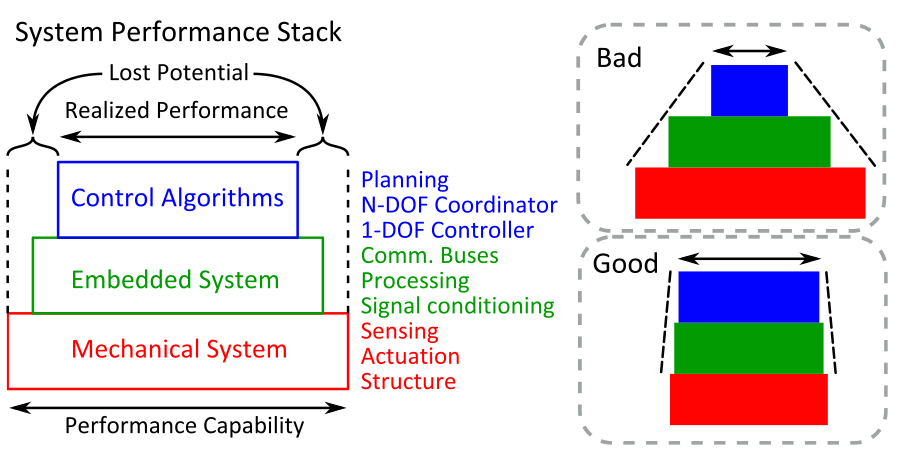
\includegraphics[width = 0.9\linewidth]{src/tex/img/system_perfomance.png}
    \caption{Representação da Capacidade de Desempenho \cite{paine2014high}}
    \label{fig:system_perfomance}
\end{figure}
\end{frame}

\section{Construção do Sistema}

\subsection{Implementação em Hardware}

\begin{frame}{Planta Simulada}
\begin{figure}
    \centering
    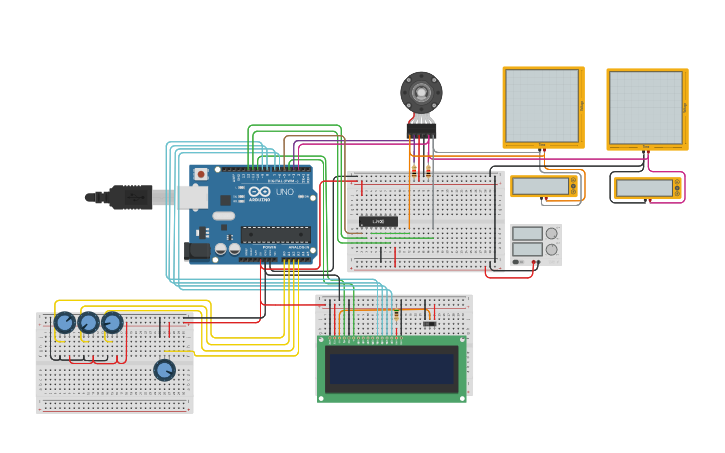
\includegraphics[width = \linewidth]{src/tex/img/pid_tinkercad.png}
    \caption{Planta no Tinkercad}
    \label{fig:control_1}
\end{figure}
\end{frame}

\begin{frame}{Planta Real}
\begin{figure}
    \centering
    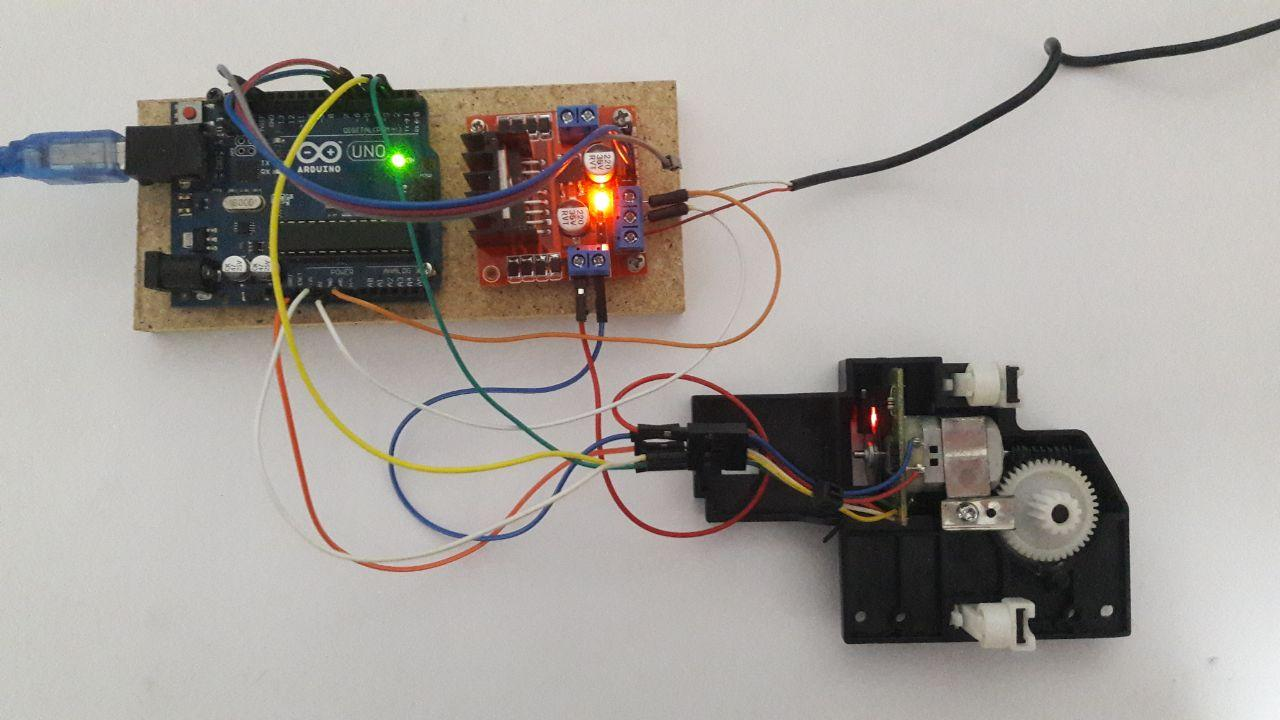
\includegraphics[width = \linewidth]{src/tex/img/full_system.jpg}
    \caption{Sistema Real}
    \label{fig:control_1}
\end{figure}
\end{frame}

\subsection{Caracterização do Sistema}

\begin{frame}{Identificação de Zona Morta}
\begin{figure}
    \centering
    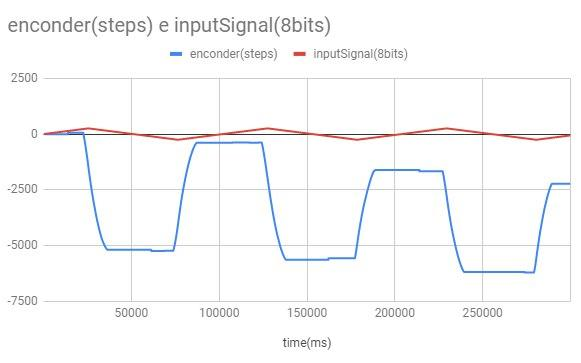
\includegraphics[width = \linewidth]{src/tex/img/grafico_dente_serra.jpg}
    \caption{Resposta do sistema para onda triangular}
    \label{fig:control_1}
\end{figure}
\end{frame}

\begin{frame}{Modelo Sistema}
    % TODO Colocar diagrama de blocos planta em malha aberta
    \begin{block}{Transformada Z}
        \begin{equation}
        G(z) = \frac{Y(z)}{U(z)} = \beta K_e \ \alpha \frac{\left(e^{-\frac{T}{\alpha} + \frac{T^2}{\alpha}}\right)z + \left(e^{-\frac{T}{\alpha}}+e^{-\frac{T}{\alpha}}\frac{T^2}{\alpha}+1\right)  }{\left(z-1\right)\left(z-e^{-\frac{T}{\alpha}}\right)}
        \label{transfdisc}
        \end{equation}
    \end{block}
\end{frame}

\begin{frame}{Identificação do Sistema}
\begin{figure}
    \centering
    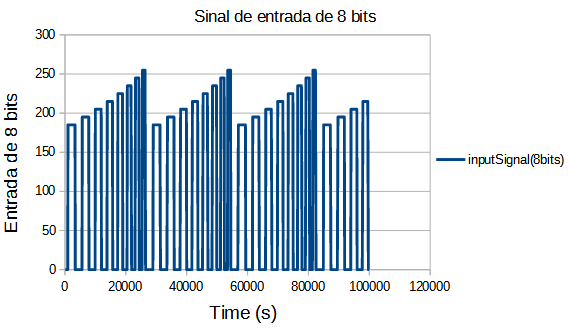
\includegraphics[width = 0.5\linewidth]{sinal_8_bits.PNG}
    \label{fig:control_1}
\end{figure}
\begin{figure}
    \centering
    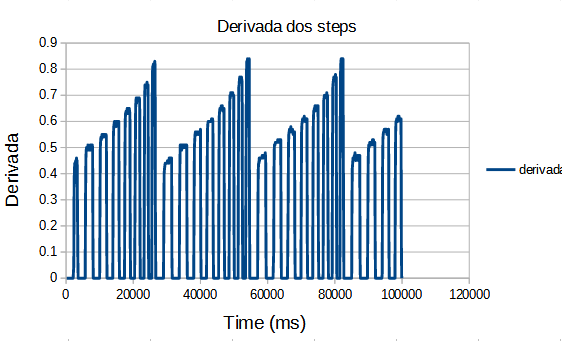
\includegraphics[width = 0.5\linewidth]{derivada_steps.PNG}
    \label{fig:control_1}
    \caption{Comparativo entre sinal de entrada e velocidade do motor}
\end{figure}
\end{frame}

\begin{frame}{Função de Transferência}
    \begin{block}{Forma Geral a partir do modelo}
        \begin{equation}\label{eq:gz_general}
            G(z) = \frac{Y(z)}{U(z)} = \frac{\beta_1 z + \beta_2}{z^2 + \alpha_1 z + \alpha_2}
        \end{equation}
    \end{block}
    
    \begin{block}{Resultado Experimental}
        \begin{equation}
        G(z) = \frac{Y(z)}{U(z)} = \frac{0.19422\,z-0.092392}{z^2-1.6576\,z+0.65762}
        \label{transfdisc}
        \end{equation}
    \end{block}
\end{frame}

\begin{frame}{Análise da resposta em frequência}
\begin{columns}
\begin{column}{0.6\textwidth}  %%<--- here
\begin{figure}
    \centering
    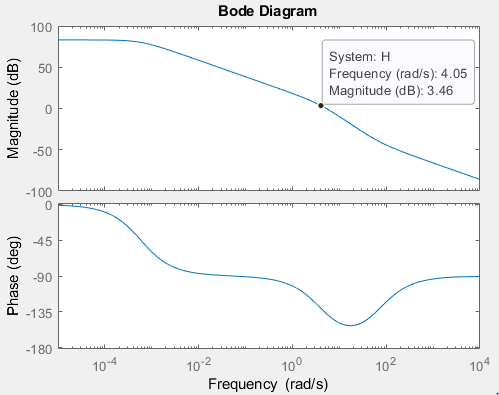
\includegraphics[width = 1.1\linewidth]{src/tex/img/bode.PNG}
    \caption{Diagrama de Bode do sistema}
\end{figure}
\end{column}
\begin{column}{0.4\textwidth}
\begin{itemize}
    \item Largura de banda bastante limitada
\end{itemize}
\end{column}
\end{columns}
\end{frame}

\section{Projeto do Controlador}
\subsection{Controle Proporcional}

\begin{frame}{LGR da planta no plano Z}
\begin{figure}
    \centering
    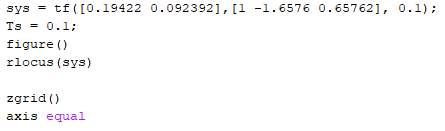
\includegraphics[width = \linewidth]{src/tex/img/script.PNG}
    \caption{Comandos no Matlab}
    \label{fig:control_1}
\end{figure}
\end{frame}

\begin{frame}{LGR da Planta no Plano Z}
\begin{figure}
    \centering
    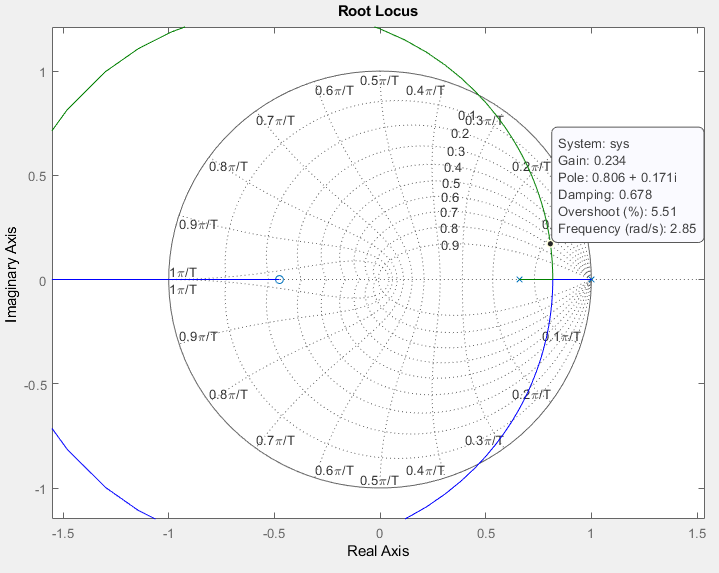
\includegraphics[width = 0.8 \linewidth]{src/tex/img/rlocus.PNG}
    \caption{Gráfico do lugar das raízes}
    \label{fig:control_1}
\end{figure}
\end{frame}

\begin{frame}{Controle Proporcional}
\begin{figure}
    \centering
    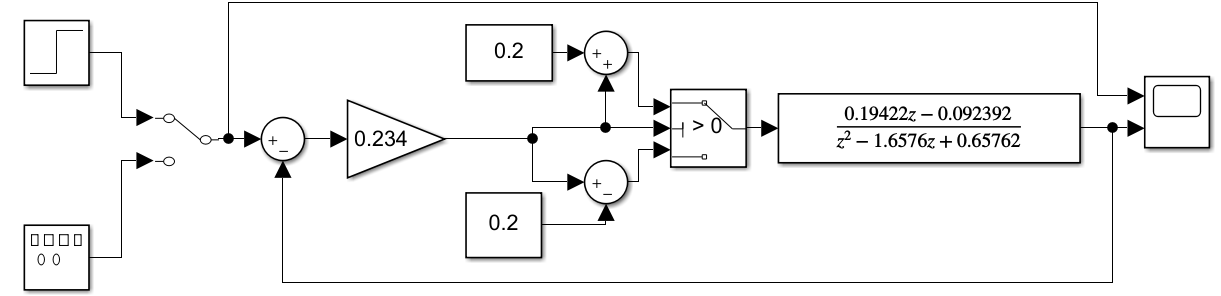
\includegraphics[width = \linewidth]{src/tex/img/controle_1.PNG}
    \caption{Diagrama de blocos do controlador proporcional}
    \label{fig:control_1}
\end{figure}
\end{frame}

\begin{frame}{Resultados do Controle Proporcional}
\begin{figure}
    \centering
    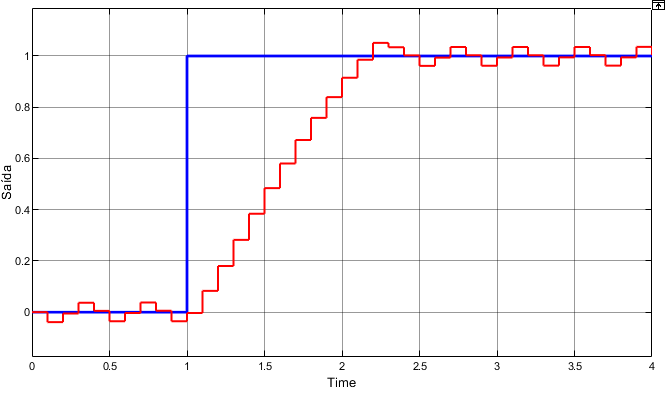
\includegraphics[width = \linewidth]{src/tex/img/saida_controle_1.png}
    \caption{Resposta ao degrau na simulação}
    \label{fig:control_1}
\end{figure}
\end{frame}


\subsection{Projeto em Frequência}

\begin{frame}{Segunda Proposta de Controlador}

Função de transferência da planta no domínio s:
\begin{equation}
G(s) = \frac{0.5011(s+70.0259)}{(s+0.00058419)(s+4.19042)}
\label{equacao_s}
\end{equation}

Estratégia: Anular o polo mais distante da planta e adicionar outro, utilizando a equação de tempo de assentamento de um sistema de segunda ordem:

\begin{equation}
\zeta \omega_{n}=\frac{4}{T_{s}}
\label{assentamento_eq}
\end{equation}

\begin{equation}
G_{c}(s)=\frac{s+4.19042}{s+8}
\label{novogc}
\end{equation}
\end{frame}

\begin{frame}{Segunda Proposta de Controlador}

\begin{figure}[H]
    \centering
    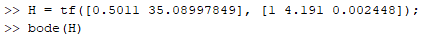
\includegraphics[width=0.7\linewidth]{src/tex/img/bode_comandos.PNG}
    \caption{Comandos no Matlab}
    \label{fig:lgr}
\end{figure}

\begin{figure}[H]
    \centering
    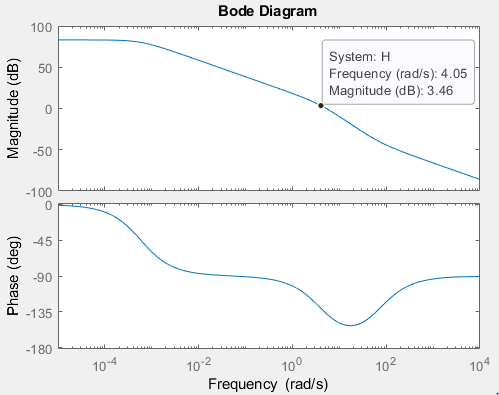
\includegraphics[width=0.6\linewidth]{src/tex/img/bode.PNG}
    \caption{Diagrama de Bode}
    \label{fig:lgr}
\end{figure}

\end{frame}



\begin{frame}{Segunda Proposta de Controlador}
Equação final do controlador:
\begin{equation}
G_{c}(z)=3.46\frac{z - 0.7116}{z - 0.4493}
\label{novogcz}
\end{equation}

\begin{figure}
    \centering
    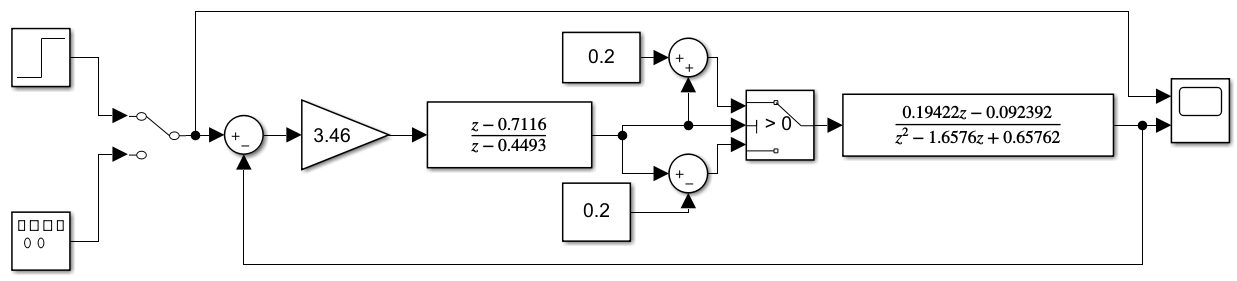
\includegraphics[width = \linewidth]{src/tex/img/controle_2.PNG}
    \caption{Diagrama de blocos do controlador 2}
    \label{fig:control_2}
\end{figure}
\end{frame}

\begin{frame}{Resultados da Segunda Proposta de Controlador}
\begin{figure}
    \centering
    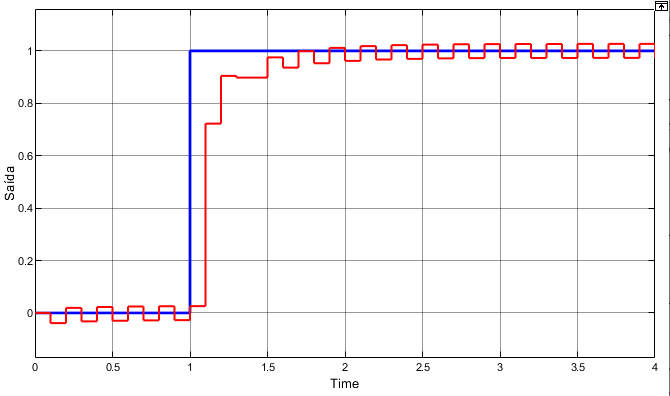
\includegraphics[width = \linewidth]{src/tex/img/saida_controle_2.png}
    \caption{Resposta ao degrau - controlador 2}
    \label{fig:controler1}
\end{figure}
\end{frame}

\begin{frame}{Resultados da Segunda Proposta de Controlador}
\begin{figure}
    \centering
    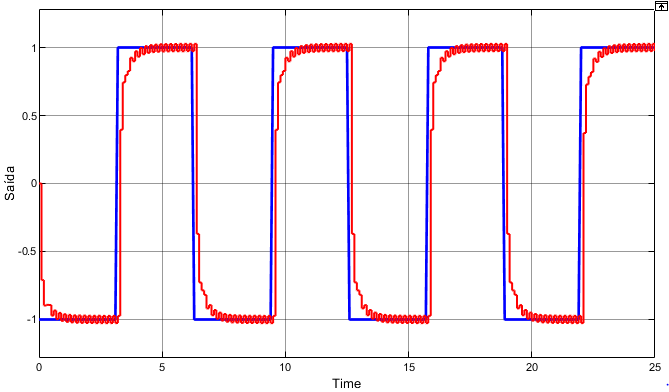
\includegraphics[width = \linewidth]{src/tex/img/teste_square.PNG}
    \caption{Resposta à onda quadrada}
    \label{fig:controler2}
\end{figure}
\end{frame}

\begin{frame}{Resposta em Hardware do Primeiro Controlador}
\begin{figure}
    \centering
    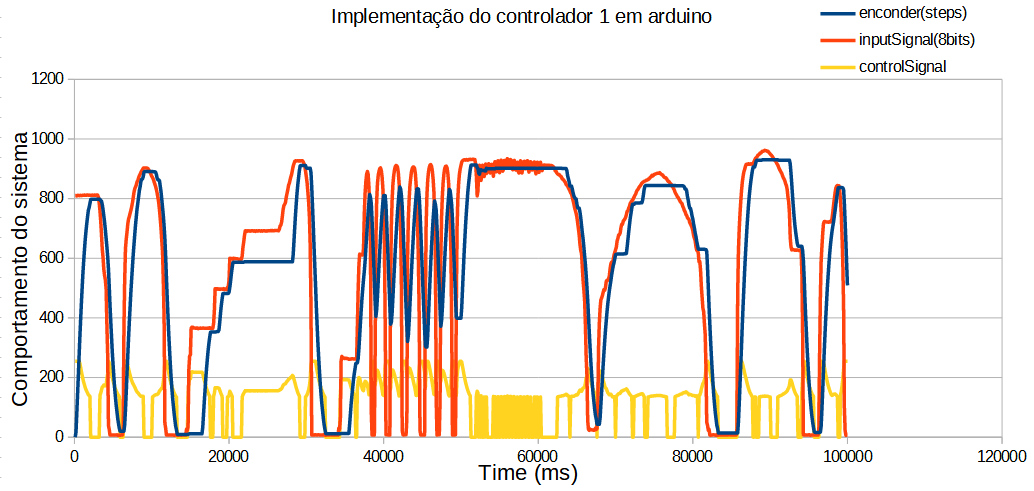
\includegraphics[width = \linewidth]{src/tex/img/resultado_controle_1_implem.PNG}
    \caption{Resposta planta - $K_p = 0.25$}
    \label{fig:control_1}
\end{figure}
\end{frame}

\section{Conclusão}

\begin{frame}{Conclusão}
\begin{itemize}
    %\item Deu tudo errado
    \item Sistema final lento;
    \item Para variações lentas, foi obtido erro estacionário baixo;
    \item Erro cumulativo da leitura de posição;
    \item Comprometimento da precisão devido à representação numérica em binário.
\end{itemize}
\end{frame}

\begin{frame}{Trabalhos Futuros}
% Modelagem Matemática
\begin{itemize}
    \item Implementação de filtros para o encoder;
    \item Projeto de controladores no espaço de estados;
    \item Projeto de PID completo;
    \item Medir tempos usando hardware externo como forma de remover a necessidade da comunicação serial;
    \item Calibrar as medidas do encoder com base em sistema externo.
\end{itemize}
\end{frame}

\begin{frame}{}
% Obrigado!
\centering
\Huge{Obrigado!}
\end{frame}

\nocite{nise2012}

\begin{frame}{Referências}
\bibliographystyle{abbrv} % Define Estilo e gera bibliografia
\bibliography{references} % Adiciona Arquivo com Referências
\end{frame}

\end{document}